In this chapter we generalize our problem to allow for partitioning $C$ into parts
that are not necessarily clone sets, but that are, nonetheless, close to being clone sets in some sense.
We formalize the measurement of distance from given partition to some decloning.
For given preference profile we try to find a partition that minimizes the distance value.

\section{General Problem}

One may claim that the \textsc{Decloning} problem is unrealistic
because it assumes that every single voter can perfectly group clones.
It disallows any error in that matter during voting, or any personal biases.
Now we drop the restriction that every part of the candidate set partition needs to be a clone set.
Instead, we will measure how far, in some sense, a given part is from being a clone set.
Of course, we require that this measure equals $0$ only for clone sets.

Let us define the clone set error function that captures this measure.
We can evaluate it on each non-empty subset of the candidate set.

\begin{defn}[clone set error function]
Let $P$ be a preference profile over candidate set $C$.
We say that a function
$f: 2^C \setminus \{\emptyset\} \rightarrow \mathbb{R}_0^+$
is a clone set error function for $P$ when $f(X) = 0$ iff $X$ is a clone set for $P$.
\end{defn}

Now we can generalize the \textsc{Decloning} problem into \textsc{OptimalDecloning},
where we try to minimize the sum of errors of parts of candidate set partition.

\begin{problem}{OptimalDecloning}
	Input: Preference profile $P$ over candidate set $C$, integer $k$, positive real number $l$,
        clone set error function $f$ encoded as a Turing machine that given input $X$ computes $f(X)$
        in at most $a \abs{X}^b$ steps for some integers $a$ and $b$

	Question: Is there a partition of $C$ into $C_1, ..., C_k$ such that $\sum_{i=1}^k f(C_i) \leq l$?
\end{problem}

\begin{thm} \label{optdecl}
	\textsc{OptimalDecloning} is \np-complete.
\end{thm}

The following lemma will be useful to prove the theorem.
It shows how to, for any candidate set, create a preference profile with no non-trivial clone sets.

\begin{lmm} \label{lmmnotrivial}
        Let $C = \{c_1, ..., c_n\}$ be any candidate set.
	Preference profle $P = (\succ_1, ... , \succ_n)$ over $C$
	where for each $i=1,...,n$ we have
	$$c_i \succ_i c_{i+1} \succ_i ... \succ_i c_n \succ_i c_1 \succ_i c_2 \succ_i ... \succ_i c_{i-1}$$
	has no non-trivial clone sets.
\end{lmm}

\begin{proof}[Proof by contradiction]
Let us consider some non-trivial clone set $X$ for $P$.
From Remark \ref{sequence-split} we have that it is a contiguous subsequence of preference order $\succ_1$,
so $X = \{c_i, ..., c_j\}$ for some $c_i, c_j \in C$.
Clone set $X$ is not trivial, so $i\neq{j}$ and $X\neq{C}$.
We note that $X$ is not contiguous on the preference order $\succ_{i+1}$.
Subset $X$ is, thus, not a clone set for $P$.
\end{proof}

The property of preference profile having no non-trivial clones lets us easily
verify whether given function is clone set error function for this preference profile.

\begin{rmrk}
Let $P$ be a preference profile over candidate set $C$
and $f : 2^C\setminus\{\emptyset\} \rightarrow \mathbb{R}_0^+$ be some function.
If $P$ has no non-trivial clones, then $f$ is clone set error function for $P$
iff for each $X \subset C$, $X \neq \emptyset$ we have that $f(X) = 0$ only when $\abs{X} \in \{1, \abs{C}\}$.
\end{rmrk}

\begin{proof}[Proof of Theorem \ref{optdecl}]
\textsc{OptimalDecloning} is clearly in \np,
as given a partition we may verify the inequality in polynomial time.
Now we only need to show that the problem is \np-hard.
We give a reduction from the \textsc{X3C} problem.

We are given set $X$, collection $S$ of 3-element subsets of $X$, and an integer $n$ such that $\abs{X} = 3n$.
Let us take candidate set $C = X$
and function $f:2^C \setminus \{\emptyset\} \rightarrow \{0,1,n+1\}$ such that:
$$ f(X) =
\begin{cases}
0, &\text{when } \abs{X} \in \{1,3n\} \text{,} \\
1, &\text{when }  X \in S \text{,} \\
n+1, &\text{otherwise.}
\end{cases}
$$
Function $f$ is well-defined when $n>1$, because if $X \in S$ then $\abs{X} = 3 \not\in \{1,3n\}$.
Trivial case $n=1$ can be treated specially during the runtime of the reduction.
Let us take preference profile $P$ over $C$ as in Lemma \ref{lmmnotrivial}.
Function $f$ is a clone set error function for $P$, because $f(X) = 0$ iff $X$ is a trivial clone set
and preference profile $P$ has no non-trivial clone sets.
Let us take $l=k=n$.
Now we have all the inputs necessary for \textsc{OptimalDecloning} problem.
Let us check when the answer to this problem is \textsc{yes}.

No part $X$ of the partition of $C$ can have $f(X)=n+1$, as it itself exceeds limit $l$.
This means that every part $X$ either belongs to $S$ or has $\abs{X} \in \{1,3n\}$.
In both cases $\abs{X} \in \{1,3,3n\}$.
When $n>1$ we cannot use $3n$-sized parts,
as it yields only one part in partition while $k>1$.

We are left with $\abs{X} \in \{1,3\}$.
Let us note that due to the specified size $k=n$ of partition and $\abs{C} = 3n$,
the partition can contain only three-element parts.
This means that we may choose $X$ only from $S$.
It is possible to construct a valid partition only when there is an $A \subset S$ satisfying the \textsc{X3C} problem.

In this case, we have partition $A$ of candidate set $C$ such that:
$$ \sum_{X \in A} f(X) = \sum_{X \in A} 1 = n,$$
so the answer to \textsc{OptimalDecloning} problem is \textsc{yes}
iff the answer to \textsc{X3C} is~\textsc{yes}.
\end{proof}



\section{Specific Error Functions}

In the proof of \np-completeness of the \textsc{OptimalDecloning} problem
we used a very artificial preference profile and error function.
Now, we will study more natural ones.

Let us try to fix a value of error function input to \textsc{OptimalDecloning} problem,
treating it as if it was hardcoded into the specification of the new problem.

Given a specific error function we will consider the following family of problems.

\begin{problem}{ $f$ Optimal Decloning}
	Input: Preference profile $P$ over $C$, integers $k$ and $l$.

	Question: Is there a partition of $C$ into $C_1, ..., C_k$ such that $\sum_{i=1}^k f(C_i) \leq l$?
\end{problem}

We want from such an error function $f$ to capture the intuitive notion
of distance of given partition from some decloning.

\subsection{Component Error Function}

We note that in decloning each clone set occurs in a contiguous part of every voter's preference order.
We may use this feature to compute clone set error for any partition.
Let the value of component error function on given part be the sum of excessive connected components
of this part in each voter's preference order.

\begin{exmp}
For a candidate set $C = \{a, b, c, d, e\}$,
let us consider a preference profile $P = (\succ_1, \succ_2, \succ_3)$ with:
\begin{align*}
a \succ_1 b \succ_1 c \succ_1 d \succ_1 e,\\
e \succ_2 d \succ_2 c \succ_2 a \succ_2 b,\\
a \succ_3 b \succ_3 e \succ_3 d \succ_3 c.
\end{align*}
The value of component error function for subset $\{b,c,e\}$ is $4$.
The subset is split into one extra piece on preference orders $\succ_1$ and $\succ_3$
($\{b,c\}, \{e\}$ and $\{b,e\}, \{c\}$ respectively),
and two extra pieces on preference order $\succ_2$ ($\{e\}, \{c\}, \{b\}$).

The error value for clone set $\{c, d, e\}$ is $0$,
because it is contiguous on each preference order.
\end{exmp}

To formulate the formal definition of component error function
we will need a definition of a kernel of a total order relation.

Given a total order $\succ$ over a finite set, we may sort its elements into a sequence
such that for every pair of elements former is in the relation $\succ$ with the latter.
This sequence naturally induces another relation, namely relation $\overline{\succ}$
between every two consecutive elements.
We will call such a relation a kernel of $\succ$.
It is easy to recover $\succ$ from $\overline{\succ}$
simply by taking the transitive closure of $\overline{\succ}$.

\begin{defn}[kernel of total order]
Given a total order $\succ$ over a finite set, we say that $\overline{\succ}$ is its kernel when
$\overline{\succ}$ is a minimal relation whose transitive closure equals $\succ$.
\end{defn}

\begin{exmp}
\sloppy
Kernel of natural order $>$ over set $\{1,2,3,4\}$ is the relation
$\overline{>} = \{(4,3), (3,2), (2,1)\}$.
\end{exmp}

\begin{defn}[component error function]
Let $P = (\succ_1, ..., \succ_m)$ be a preference profile over candidate set $C$.
We define component error function for $P$ as
a function $f_{com}: 2^C \setminus \{\emptyset\} \rightarrow \mathbb{N}_0$ with the following formula:
$$ f_{com}(X) = \sum_{i=1}^m \left( \abs{X}-1 -
\abs{\left\lbrace \left( a,b \right) \in X^2 : a \overline{\succ}_i b \right\rbrace }
\right) \text{.}$$
\end{defn}

\begin{rmrk}
Component error function $f_{com}$ for preference profile $P$ is a clone set error function for $P$.
\end{rmrk}

Now we may formulate optimal decloning problem that uses component error function.

\begin{problem}{ComponentOptimalDecloning (COD)}
	Input: Preference profile $P$ over $C$, integers $k$ and $l$.

	Question: Given than $f_{com}$ is a component error function for $P$,
		is there a partition of $C$ into $C_1, ..., C_k$ such that $\sum_{i=1}^k f_{com}(C_i) \leq l$?
\end{problem}

We will express this problem in a language of graph theory.

Given a preference profile $P = (\succ_1, ..., \succ_m)$ over candidate set $C$,
let us create a multigraph $G=(C,E)$.
Let $E$ be the multiset union of sets
$\left\lbrace \left\lbrace a,b \right\rbrace: a \succ_i b \right\rbrace$ for $i=1, ..., m$.
We got a multigraph created from multiset union of edges of some Hamiltonian paths,
for each voter's preference order.
Let us call this a Hamiltonian path multigraph.

\begin{defn}[Hamiltonian path multigraph]
A multigraph $G=(V,E)$ is a Hamiltonian path multigraph if there exists a partition of $E$
into sets of edges of Hamiltonian paths in $G$.
\end{defn}

Partitioning candidate set $C$ into $C_1,...,C_k$ corresponds to
partitioning Hamiltonian path multigraph $G$ into submultigraphs $G_1,...,G_k$
% necessary induced graphs? maybe just partition of V?
induced by $C_1,...,C_k$ respectively.
Let us denote by number $c_{ij}$ part
$\abs{\left\lbrace \left( a,b \right) \in C_i^2 : a \overline{\succ}_j b \right\rbrace }$
of the formula of $f_{com}(C_i)$, so
$f_{com}(C_i) = \sum_{j=1}^m \left( \abs{C_i} - 1 - c_{ij} \right)$.
We have that $c_{ij}$ is the number of edges from $j$-th voter's Hamiltonian path
that connect two vertices from $C_i$.
We will call such edges the $C_i$ intra-part edges.
We will also call edges that end in different parts the inter-part edges.

Now the error value equals:
$$
\sum_{i=1}^k f_{com}(C_i) =
\sum_{i=1}^k \sum_{j=1}^m \left( \abs{C_i} - 1 - c_{ij} \right) =
m \sum_{i=1}^k \abs{C_i} - m k - \sum_{i=1}^k \sum_{j=1}^m c_{ij} =
m(n-k) - \sum_{j=i}^m \sum_{i=1}^k c_{ij}
\text{.}$$

Let us note that $\sum_{i=1}^k c_{ij}$ is the total number of $C_i$ intra-part edges
and $\sum_{j=i}^m \sum_{i=1}^k c_{ij}$ is the total number of intra-part edges.
As value of $m(n-k)$ is constant for a given graph,
we have that \textsc{ComponentOptimalDecloning} is, essentially, a problem of maximizing the number of intra-part edges.
We will call that number a score of partition.

\begin{defn}[partition score]
Let $G=(V,E)$ be a multigraph, where $E=(D, e)$ for some edge set $D$,
and let $(V_1, ..., V_k)$ be a partition of $V$.
We say that a score of part $V_i$ for $i=1,...,k$ equals $\sum_{u,v \in V_i} e(\{u,v\})$.
We say that a partition score is a sum of the scores of its parts.
\end{defn}

\begin{rmrk}
Score of a part that is a singleton equals $0$.
\end{rmrk}

This lets us formulate another problem, which is polynomially reducible
to \textsc{ComponentOptimalDecloning}.

\begin{problem}{HamiltonianPathMultigraphPartition (HPMP)}
	Input: Hamiltonian path multigraph $G=(V,E)$
		together with its partition into Hamiltonian paths, integers $k$ and $s$.

	Question: Is there a partition of $V$ into $V_1, ..., V_k$,
        of score at least $s$?
\end{problem}

\begin{thm} \label{hpmp-to-cod}
There is a polynomial-time reduction of problem \textsc{HPMP} to \textsc{COD}.
\end{thm}

\begin{proof}
Given $G=(V,E)$ from the input, we take candidate set $C=V$.
For each Hamiltonian path from the input, we add to the output preference profile $P$
the preference order created by transitive closure of relation of vertices being consecutive on a path.
We have previously shown that resulting instance of the \textsc{COD} problem 
has the same answer as the input instance of \textsc{HPMP} problem.
\end{proof}


\begin{thm} \label{ultimate-theorem}
\textsc{ComponentOptimalDecloning} is \np-complete.
\end{thm}

We will prove that with a reduction of the \textsc{Clique} problem to the \textsc{HPMP} problem
(and using Theorem \ref{hpmp-to-cod} to further reduce to the \textsc{COD} problem).
To do that, we will construct from the \textsc{Clique} problem instance
a Hamiltonian path multigraph with special properties.
The following lemma uses these properties to reason on the answer to the original \textsc{Clique} problem instance.

\begin{lmm} \label{hpmp-red}
Let graph $G = (V, E)$ and integer $c$ be an instance of the \textsc{Clique} problem.
Let $G'=(V',E')$,  be a Hamiltonian path multigraph
such that $V' \supset V$, $E'=(\{\{u,v\}: u,v \in V'\}, w)$, and
$$ w(\{u,v\}) =
\begin{cases}
2, 				&\text{when } \{u,v\} \in E ,\\
0, 				&\text{when } \{u,v\} \not\in E \text{ and } u,v \in V ,\\
w_{u v}\leq 1,	&\text{when } u \not\in V \text{ or } v \not\in V.
\end{cases}
$$
There is a clique of size $c$ in $G$ iff
there is $\left(\abs{V'}-c-1\right)$-sized partition of $V'$ of score $c(c-1)$.
\end{lmm}

\begin{proof}
Let us consider graph $G=(V,E)$ and multigraph $G'=(V',(\{\{u,v\}: u,v \in V'\},w))$,
satisfying the condition of the lemma.
If there is a $c$-sized clique $C \subset V$ in $G$,
then we may partition $V'$ into $C$ and singletons for each $u \in V' \setminus C$.
As $f(\{u,v\})=2$ for $u,v \in C$, such a partition has score $2 {c(c-1) \over 2} = c(c-1)$.
This proves the implication in one direction.

Now let us study the case when there is no $c$-sized clique in $G$.
Let us consider any partition $P$ of $V'$, $P=(V_1, ..., V_k)$ for $k = \abs{V'}-c-1$.
Partition $P$ cannot contain any part bigger than $c$,
because all of the parts need to be non-empty.
If $P$ contains $c$-sized part $V_1$ included entirely in $V$, then its score is less than $c(c-1)$,
for $V$ does not contain $c$-sized cliques.
In other case, part $V_1$ contains a vertex from $V' \setminus V$.
This means that there is an edge $e$ with one vertex in $V_1$ such that $w(e) \leq 1$,
so the score of $P$ is smaller that $c(c-1)$.

The only case left is when each part of $P$ has size smaller than $c$.
We will do reasoning similar to the one in the proof of Theorem \ref{gp-np}.
Let us denote the upper bound of the score of $m$-sized part of $f(m)$, $f(m) = m(m-1)$.
Function $f$ is strictly convex because $f''(x) = 2 > 0$
and sequence $(c,1,...,1)$ majorizes sequence $S$ of sizes of $V_1, ..., V_k$,
so we can use inequality from Theorem \ref{thm:Kar}
for $f$ and both sequences.
This gives us the following upper bound on the score $q$ of $P$:
$$q \leq \sum_{s \in S} f(s) < f(c) + f(1) + ... + f(1) = c(c-1) \text{.}$$
So, also in this case the score of $P$ is smaller than $c(c-1)$ and the lemma is proved.
\end{proof}

Now we need to show that these properties are feasible,
i.e., we can compute a multigraph that satisfies them.

\begin{lmm} \label{hpmp-red-2}
Given a $(G, c)$ instance of the \textsc{Clique} problem,
there is a polynomial-time construction
of Hamiltonian path multigraph $G'$ together with its path decomposition
satisfying the conditions of Lemma \ref{hpmp-red}.
\end{lmm}

\begin{proof}
Let $G = (V,E)$, $V = \{v_1, ..., v_n\}$ and $E = \{\{v_{e_i}, v_{d_i}\}: i = 1, ..., m\}$,
$e_i < d_i$ for $i=1,...,m$.
We need a prime number $p > 8m^2 n$.
Using Theorem \ref{bertrand-chebyshev} we have that there exists a prime number between $8m^2n$ and $16m^2 n$.
This lets us find $p$ using a brute-force linear search.

\sloppy
We will construct Hamiltonian path multigraph $G' = (V',E')$
with $V' = \{v_1, ..., v_n, v_{n+1}, ..., v_{n+p}\}$. 
Now we create $2m$ paths, where the $i$-th path for $i=1,...,2m$
is formed by the following sequence $P_i$ of vertices:
$$ P_i = ({P_i}_1, ..., {P_i}_p) =  (v_{n+1+(ji \mod p)})_{j=1,...,p} \text{.}$$ 
From Theorem \ref{zp} we have that each such path has every vertex from
$V' \setminus V = \{v_{n+1}, ..., v_{n+p}\}$.
We also note that the paths do not share edges,
because if the $i$-th path contains edge $\{v_a, v_b\}$, then $\abs{a-b} = i$.

To make them Hamiltonian paths we need to extend them with the vertices from $V$.
Let us create $2m$ permutations $S_i$ of $V$ for $i=1,...,2m$ such that
$$S_i = ({S_i}_{,1}; ...; {S_i}_{,n}) =
(v_{e_i}, v_{d_i}, v_1, ..., v_{e_i-1}, v_{e_i+1}, ..., v_{d_i-1}, v_{d_i+1}, ..., v_n)\text{,}$$
where we denote $v_{e_i} = v_{e_{i-m}}$ and $v_{d_i} = v_{d_{i-m}}$ for $i>m$. 

Now we merge sequences $P_i$ and $S_i$ for $i=1,...,2m$ respectively to obtain Hamiltonian paths.
Sequence $H_i$ of vertices of the $i$-th Hamiltonian path looks as follows:
$$H_i = ({P_i}_{,1}; ...; {P_i}_{,1+ni}; {S_i}_{,1}; {S_i}_{,2}; {P_i}_{,2+ni}; {S_i}_{,3}; ...;
{P_i}_{,n-1+ni}; {S_i}_{,n}; {P_i}_{,n+ni}; ...; {P_i}_{,p}) \text{.}$$

\begin{figure}[h]
    \centering
    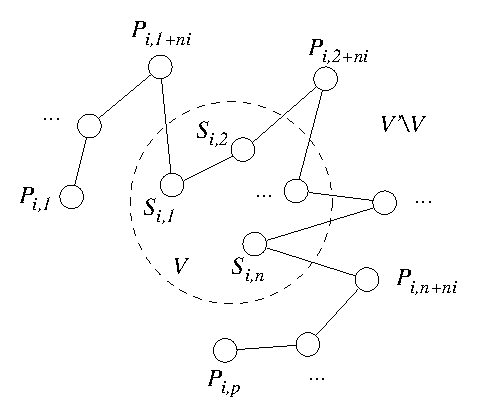
\includegraphics[width=0.4\textwidth]{path.eps}
    \caption{Sequence $H_i$ of vertices of $i$-th Hamiltonian path.}
    \label{fig:path}
\end{figure}

We get a path as depicted on Figure \ref{fig:path}.

What happened here is that we put $1+ni$ first vertices from $P_i$,
put two first vertices from $S_i$, merged next vertices from $P_i$ and $S_i$ one to one,
and put remaining vertices from $P_i$.
In the sequence $H_i$ there are edges between vertices from $P_i$ and $S_i$
only for vertices ${P_i}_{,1+ni}; ...; {P_i}_{,n+ni}$ in $P_i$.
These are vertices $v_{n+1+((1+ni)i \mod p)}, ..., v_{n+((n+1+ni)i \mod p)} $.
As $i \leq 2m$, then $(n+1+ni)i \leq (mn+mn+2mn)2m = 8m^2 n < p$,
so we may remove modulo operations from those indices.
Now for $H_i$ we have vertices $v_{n+1+i+ni^2}, ..., v_{n+ni+i+ni^2}$.
We note that for each $i=1,...,2m$ those vertices are disjoint,
so no edge between $V$ and $V' \setminus V$ appears twice.

The resulting Hamiltonian paths have the following properties:
\begin{itemize}
\item each contains one edge from $E$ with both ends in $V$,
  and each edge in $E$ appears in two paths,
\item no two paths share a common edge with both ends in $V' \setminus V$,
  i.e., for each $u,v \in V' \setminus V$ edge $\{u,v\}$ appears at most once,
\item the same holds for vertices $u,v$ such that $u \in V$, $v \in V' \setminus V$.
\end{itemize}
This means that we constructed a required multigraph, together with its decomposition into paths.
\end{proof}

Using the previous two lemmas, we are ready to prove our theorem.

\begin{proof}[Proof of Theorem \ref{ultimate-theorem}.]
We will show a reduction from \textsc{Clique} problem to \textsc{HPMP}.
We are given graph $G = (V, E)$ and integer $c$.
Lemma \ref{hpmp-red-2} shows a polynomial-time construction of Hamiltonian path multigraph $G'$,
such that $V' \supset V$, $E'=(\{\{u,v\}: u,v \in V'\}, w)$, and
$$ w(\{u,v\}) =
\begin{cases}
2, 				&\text{when } \{u,v\} \in E ,\\
0, 				&\text{when } \{u,v\} \not\in E \text{ and } u,v \in V ,\\
w_{u v}\leq 1,	&\text{when } u \not\in V \text{ or } v \not\in V.
\end{cases}
$$
Let us take $k=\abs{V'}-c-1$ and $s=c(c-1)$, what gives us full instance of the \textsc{HPMP} problem.
From Lemma \ref{hpmp-red} follows that there is a $c$-sized clique in $G$
iff there is a $k$-sized partition of $V'$ of score $s$.
This means it is a valid reduction from the \textsc{Clique} problem to \textsc{HPMP}.
Using Theorem \ref{hpmp-to-cod} we can reduce it further to the \textsc{COD} problem.

We have shown a reduction from \np-complete problem to the \textsc{COD} problem,
and \textsc{COD} is clearly in \np.
From this follows that the \textsc{COD} problem is \np-complete.
\end{proof}


\subsection{Inconsistent Voters Error Function}

Component error function has useful properties, but also could yield partitions
intuitively far from optimal.
It constructs the partition using only very local information,
such as edges in the graphs of kernels of preference orders.
For example, in the proof of Theorem \ref{ultimate-theorem}, we constructed a partition
which was not in accordance with any voter.

On the other side of the spectrum of locality, we may think of an error function which
takes into consideration only global information, in the sense of a single voter.
Such an information is what we call consistency with a voter's preferences, that we define below.

\begin{defn}[inconsistent voter]
We say that a voter described by preference order~$\succ$ over $C$
is consistent with a non-empty subset $X \subset C$
iff $X$ is a clone set for preference profile $P = (\succ)$.
We also say that $\succ$ is inconsistent with $X$ if it is not consistent with $X$.
\end{defn}

\begin{defn}[inconsistent voters error function]
Given a preference profile $P$ over $C$ we define function
$f_{iv}: 2^C \setminus \{\emptyset\} \rightarrow \mathbb{N}_0$ so that
$f(X)$ is the number of preference orders in $P$ that are inconsistent with $X$.
\end{defn}

\begin{rmrk}
Function $f_{iv}$ for preference profile $P$ is a clone set error function for $P$.
\end{rmrk}

Now we can introduce optimal decloning problem using $f_{iv}$ clone set error function.

\begin{problem}{ConsistentVotersOptimalDecloning (CVOD)}
	Input: Preference profile $P$ over $C$, integers $k$ and $l$.

	Question: Given than $f_{iv}$ is the inconsistent voters error function for $P$,
		is there a partition of $C$ into $C_1, ..., C_k$ such that $\sum_{i=1}^k f_{iv}(C_i) \leq l$?
\end{problem}

\begin{rmrk}
\textsc{CVOD} problem is in \np.
\end{rmrk}

It remains an open problem whether \textsc{CVOD} problem is \np-complete.
